\documentclass[epsfig,10pt,fullpage]{article}

\newcommand{\LabNum}{5}
\newcommand{\CommonDocsPath}{../../../../common/docs}
\addtolength{\textwidth}{1.5in}
\addtolength{\oddsidemargin}{-0.75in}
\addtolength{\topmargin}{-0.75in}
\addtolength{\textheight}{1.5in}
\addtolength{\evensidemargin}{0.75in}
\setlength\parindent{0pt}
\raggedbottom

\usepackage{ae,aecompl}
\usepackage{epsfig,float,times}
\usepackage[hypcap]{caption}
\usepackage[pdftex, colorlinks]{hyperref}
\usepackage{graphicx}
\usepackage[usenames, dvipsnames]{color}
\usepackage{rotating}
\usepackage{tikz}
\usetikzlibrary{automata,positioning}
\usepackage{placeins}

\widowpenalty 10000
\clubpenalty 10000

\newcommand{\red}[1]{{\color{red}\sf{#1}}}
\newcommand{\green}[1]{{\color{green}\sf{#1}}}
\newcommand{\blue}[1]{{\color{blue}\sf{#1}}}
\definecolor{PineGreen}{rgb}{0.0, 0.47, 0.44}
\definecolor{ForestGreen}{rgb}{0.13, 0.55, 0.13}
\definecolor{Brown}{rgb}{0.59, 0.29, 0.0}

\newcommand{\UPDatePublished}{Oct 2021}
\newcommand{\versnum}{21.1} %version number quartus/AMP
\newcommand{\quartusname}{Quartus\textsuperscript{\textregistered} Prime}	
\newcommand{\UPTextBar}{For \quartusname{} \versnum{}}
\newcommand{\thisyear}{2021 } %for copyright
\newcommand{\company}{FPGAcademy.org}
\newcommand{\longteamname}{FPGAcademy.org}
\newcommand{\teamname}{FPGAcademy}
\newcommand{\website}{FPGAcademy.org}

\newcommand{\productAcronym}{AMP}
\newcommand{\productNameShort}{Monitor Program}

\newcommand{\productNameMedTM}{A Monitor Program}
\newcommand{\productNameMed}{A Monitor Program}

%\newcommand{\headerLogoFilePath}[1]{#1/FPGAcademy.png}

% listings is a package that supports encapsulating source code in LaTeX conveniently
\usepackage{listings}

\def\expandparam\lstinputlisting[#1]#2{\edef\tmp{\noexpand\lstinputlisting[#1]{#2}}\tmp}

%%%%%%%%%%%%%%%%%%%% Source Code Formatting %%%%%%%%%%%%%%%%%%%%
\definecolor{globalCommentColour}{rgb}{0.588,0.588,0.588}

%%%%%%%%%%%%%%%%%%%%%%%%%%%%%%%%%%%%%%%%%%%%%%%%%%%%
% Defining language style
% NiosII ASM
\lstdefinelanguage[NiosII]{Assembler} {
  morekeywords={add, addi, and, andhi, andi, beq, bge, bgeu, bgt, bgtu, ble,  bleu, blt, bltu, bne, br, break,
  bret, call, callr, cmpeq, cmpeqi, cmpge, cmpgei, cmpgeu, cmpgeui, cmpgt, cmpgti, cmpgtu, cmpgtui, cmple,
  cmplei, cmpleu, cmpleui, cmplt, cmplti, cmpltu, cmpltui, cmpne, cmpnei, custom, div, divu, eret, flushd,
  flushda, flushi, flushp, initd, initda, initi, jmp, jmpi, ldb, ldbio, ldbu, ldbuio, ldh, ldhio, ldhu, ldhuio,
  ldw, ldwio, mov, movhi, movi, movia, movui, mul, muli, mulxss, mulxsu, mulxuu, nextpc, nop, nor, or, orhi, ori,
  rdctl, rdprs, ret, rol, roli, ror, sll, slli, sra, srai, srl, srli, stb, stbio, sth, sthio, stw, stwio,
  sub, subi, sync, trap, wrctl, wrtcl, wrprs, xor, xori, xorhi, xori},
  morekeywords=[2]{.abort, .ABORT, .align, .app-file, .ascii, .asciz, .balign, .byte, .comm, .data, .def,
  .desc, .dim, .double, .eject, .else, .end, .endef, .endif, .equ, .equiv, .err, .extern, .file, .fill, .float,
  .global, .globl, .hword, .ident, .if, .include, .int, .irp, .irpc, .lcomm, .lflags, .line, .linkonce, .ln,
  .list, .long, .macro, .mri, .nolist, .octa, .org, .p2align, .psize, .quad, .rept, .sbttl, .scl, .section,
  .set, .short, .single, .size, .sleb128, .skip, .space, .stadb, .stabn, .stabs, .string, .symver, .tag,
  .text, .title, .type, .val, .uleb128, .word},
  morekeywords=[3]{et, bt, gp, sp, fp, ea, sstatus, ra, pc, status, estatus, bstatus, ienable, ipending, cpuid,
  exception, pteaddr, tlbacc, tlbmisc, eccinj, badaddr, config, mpubase, mpuacc},
  sensitive=t,
  alsoletter=.,
  morestring=[b]",
  morecomment=[s]{/*}{*/},
  morecomment=[l]\#,
}[keywords,comments,strings]
   
%% NOTE: morekeywords=[2] are GNU directives.
   
\definecolor{niosInstructionColour}{rgb}{0.000,0.608,0.000}
\definecolor{niosDirectiveColour}{rgb}{0.000,0.000,0.902}
\definecolor{niosSpecialRegColour}{rgb}{0.000,0.000,0.000}
\definecolor{niosStringColour}{rgb}{0.808,0.482,0.000}
   
%% NOTE: To make bold use: =\bfseries\color{<colour>}
\lstdefinestyle{defaultNiosStyle} {
  language=[NiosII]{Assembler},
  stringstyle=\color{niosStringColour},
  keywordstyle=\color{niosInstructionColour},
  keywordstyle=[2]\color{niosDirectiveColour},
  keywordstyle=[3]\itshape\color{niosSpecialRegColour}
}
%%%%%%%%%%%%%%%%%%%%%%%%%%%%%%%%%%%%%%%%%%%%%%%%%%%%

%%%%%%%%%%%%%%%%%%%%%%%%%%%%%%%%%%%%%%%%%%%%%%%%%%%%
% Defining language style
% ArmA9 ASM
\lstdefinelanguage[ArmA9]{Assembler} {
  morekeywords={ADC, ADD, ADDS, AND, ANDS, B, BAL, BEQ, BGE, BGT, BL, BLT, BIC, BKPT, BLX, BNE, BX, CDP, CLZ, CMN, CMP, EOR,
  EORS, LDC, LDM, LDR, LDRB, LDRBT, LDRH, LDRSB, LDRSH, LDRT, LSL, MCR, MLA, MOV, MOVW, MOVT, MRC, MRS, MSR, MUL, MVN, ORR, PLD,
  ROR, RSB, RSC, SBC, SMLAL, SMULL, STC, STM, STR, STRB, STRBT, STRH, STRT, SUB, SUBS, SWI, SWP, SWPB, TEQ, UMLAL,
  PUSH, POP, MOVS, RORS, LSR},
  morekeywords=[2]{.abort, .ABORT, .align, .app-file, .ascii, .asciz, .balign, .byte, .comm, .data, .def,
  .desc, .dim, .double, .eject, .else, .end, .endef, .endif, .equ, .equiv, .err, .extern, .file, .fill, .float,
  .global, .globl, .hword, .ident, .if, .include, .int, .irp, .irpc, .lcomm, .lflags, .line, .linkonce, .ln,
  .list, .long, .macro, .mri, .nolist, .octa, .org, .p2align, .psize, .quad, .rept, .sbttl, .scl, .section,
  .set, .short, .single, .size, .sleb128, .skip, .space, .stadb, .stabn, .stabs, .string, .symver, .tag,
  .text, .title, .type, .val, .vectors, .uleb128, .word},
  morekeywords=[3]{SP, PC, MIDR, CTR, TCMTR, TLBTR, MPIDR, ID_PFR0, ID_PFR1, ID_DFR0, ID_MMFR0, ID_MMFR1, ID_MMFR2,
  ID_MMFR3, ID_ISAR0, ID_ISAR1, ID_ISAR2, ID_ISAR3, ID_ISAR4, CCSIDR, CLIDR, AIDR, CSSELR, TTBR0, TTRB1, TTBR2, DACR,
  DFSR, IFSR, ADFSR, AIFSR, DFAAR, IFAR, ICIALLUIS, BPIALLIS, PAR, ICIALLU, ICIMVAU, BPIALL, DCIMVAC, DCISW, V2PCWPR,
  DCCVAC, DCCSW, DDIMVAC, DCISW, TLBALLIS, TLBIMVAIS, TLBIASIDIS, TLBIMVAAIS, TLBIALL, TLBIMVA, TLBIASID, TLBIMVAA,
  PMCR, PMCNTENSET, PMCNTENCLR, PMOVSR, PMSWINC, PMSELR, PMXEVTYPER, PMXEVCNTR, PMUSERENR, PMINTENSET, PMINTENCLR,
  PRRR, NRRR, PLEIDR, PLEASR, PLEFSR, PLEUAR, PLEPCR, VBAR, MVBAR, ISR, FCSEIDR, CONTEXTIDR, TPIDRURW, TPIDRURO, TPIDRPRW},
  sensitive=f,
  alsoletter=.,
  morestring=[b]",
  morecomment=[s]{/*}{*/},
  morecomment=[l]{//},
}[keywords,comments,strings]
   
%% NOTE: morekeywords=[2] are GNU directives.
   
\definecolor{armInstructionColour}{rgb}{0.000,0.608,0.000}
\definecolor{armDirectiveColour}{rgb}{0.000,0.000,0.902}
\definecolor{armSpecialRegColour}{rgb}{0.000,0.000,0.000}
\definecolor{armStringColour}{rgb}{0.808,0.482,0.000}
   
\lstdefinestyle{defaultArmStyle} {
  language=[ArmA9]{Assembler},
  stringstyle=\color{armStringColour},
  keywordstyle=\color{armInstructionColour},
  keywordstyle=[2]\color{armDirectiveColour},
  keywordstyle=[3]\itshape\color{armSpecialRegColour}
}
%%%%%%%%%%%%%%%%%%%%%%%%%%%%%%%%%%%%%%%%%%%%%%%%%%%%

%%%%%%%%%%%%%%%%%%%%%%%%%%%%%%%%%%%%%%%%%%%%%%%%%%%%
% Defining language style
% FPGAcademy ASM
\lstdefinelanguage{ASM}{
  morekeywords = [1]{mv, mvt, mvne, mvcc, add, sub, st, ld, and, b, bne, beq, bcc, bcs},
  morekeywords = [2]{word, define},
  keywordstyle = [1]\color{ForestGreen},
  keywordstyle = [2]\color{blue},
  sensitive = true,
  morecomment = [l]{//},
}

\lstset{
  language = ASM,
  basicstyle=\small\color{black}\ttfamily,
  commentstyle=\small\color{Brown}\itshape\ttfamily,
  showstringspaces=false,
  frame=none, %lines % boxed listings
  breaklines=true,
  breakatwhitespace=true,
  tabsize=3
}
%%%%%%%%%%%%%%%%%%%%%%%%%%%%%%%%%%%%%%%%%%%%%%%%%%%%

%%%%%%%%%%%%%%%%%%%%%%%%%%%%%%%%%%%%%%%%%%%%%%%%%%%%
% Defining language style
% Java
\definecolor{javaStringColour}{rgb}{0.808,0.482,0}
%%%%%%%%%%%%%%%%%%%%%%%%%%%%%%%%%%%%%%%%%%%%%%%%%%%%

%%%%%%%%%%%%%%%%%%%%%%%%%%%%%%%%%%%%%%%%%%%%%%%%%%%%
% Defining language style
% C
\definecolor{CStringColour}{rgb}{0.808,0.482,0}

\lstset{
  language = C,
  basicstyle=\small\color{black}\ttfamily, 
  commentstyle=\small\color{PineGreen}\itshape\ttfamily,
  keywordstyle=\small\color{blue}\bfseries\ttfamily,
  showstringspaces=false,
  frame=none, %lines % boxed listings
  breaklines=true,
  breakatwhitespace=true,
  tabsize=3
}
%%%%%%%%%%%%%%%%%%%%%%%%%%%%%%%%%%%%%%%%%%%%%%%%%%%%

%%%%%%%%%%%%%%%%%%%%%%%%%%%%%%%%%%%%%%%%%%%%%%%%%%%%
% Defining language style
% Verilog
\definecolor{verilogCommentColour}{rgb}{0.000,0.502,0.000}

\lstdefinestyle{defaultVerilogStyle} {
  language={Verilog},
  keywordstyle=\color{blue},
  commentstyle=\color{verilogCommentColour}
}
%%%%%%%%%%%%%%%%%%%%%%%%%%%%%%%%%%%%%%%%%%%%%%%%%%%%

%%%%%%%%%%%%%%%%%%%%%%%%%%%%%%%%%%%%%%%%%%%%%%%%%%%%
% Defining language style
% VHDL
\lstdefinestyle{defaultVHDLStyle} {
  language={VHDL},
  keywordstyle=\color{blue},
  commentstyle=\color{verilogCommentColour}
}
%%%%%%%%%%%%%%%%%%%%%%%%%%%%%%%%%%%%%%%%%%%%%%%%%%%%

%%%%%%%%%%%%%%%%%%%%%%%%%%%%%%%%%%%%%%%%%%%%%%%%%%%%
% Defining language style
% LaTeX
\lstdefinelanguage[LocalLaTeX]{TeX}[LaTeX]{TeX}{moretexcs={bf, it, sf, lstset},}

\lstdefinestyle{defaultLocalLatexStyle} {
  language=[LocalLatex]{TeX},
  keywordstyle=\color{blue}\bfseries,
  keywordstyle=[2]\color{blue},
  keywordstyle=[3]\color{blue}\bfseries
}
%%%%%%%%%%%%%%%%%%%%%%%%%%%%%%%%%%%%%%%%%%%%%%%%%%%%

%%%%%%%%%%%%%%%%%%%%%%%%%%%%%%%%%%%%%%%%%%%%%%%%%%%%
% Defining language style
% Default
\lstset{
  basicstyle=\small\color{black}\ttfamily,
  commentstyle=\small\color{globalCommentColour}\itshape\ttfamily,
  keywordstyle=\small\color{blue}\bfseries\ttfamily,
  showstringspaces=false,
  frame=none, %lines % boxed listings
  breaklines=true,
  breakatwhitespace=true,
  tabsize=3
}
%%%%%%%%%%%%%%%%%%%%%%%%%%%%%%%%%%%%%%%%%%%%%%%%%%%%


\hypersetup{
  pdftitle={Computer Organization Lab Exercise \LabNum},
  linkcolor=blue,
  hyperindex=true,
  pdfauthor={FPGAcademy.org},
  pdfkeywords={FPGAcademy.org, FPGAcademy, Lab, Exercise, Computer Organization},
  bookmarks,
  bookmarksopen=false,
  filecolor=blue,
  pdfstartview={FitH},
  urlcolor=blue,
  plainpages=false,
  pdfpagelabels=true,
  linkbordercolor={1 1 1} %no color for link border
}



\begin{document}

\centerline{\huge Computer Organization}
~\\
\centerline{\huge Laboratory Exercise \LabNum}
~\\
\centerline{\large Using Interrupts with Assembly Code}
~\\

The purpose of this exercise is to investigate the use of interrupts for the Nios\textsuperscript{\textregistered} II
processor, using assembly-language code. To do this exercise you need to be familiar with
the exceptions processing mechanisms for the Nios~II processor, which are discussed in the 
tutorial {\it Nios~II Introduction}, available in the Intel\textsuperscript{\textregistered} PSG University Program website.
You should also read the information on exceptions and interrupts of the 
pre-built computer system documentation corresponding to which DE-series board you own.

\section*{Part I}
\addcontentsline{toc}{1}{Part I}
Consider the main program shown in Figure~\ref{fig:code}.  The main program needs to set up the 
stack pointer, configure the pushbutton KEYs port to generate interrupts, and then 
enable interrupts in the Nios~II processor.  You are to fill in the code that is not shown 
in the figure.  

~\\
The function of your program is to show the numbers \red{0} to \red{3} on the {\it HEX}0
to {\it HEX}3 displays, respectively, when a corresponding pushbutton {\it KEY} is pressed. 
Since the main program simply ``idles'' in an endless loop, as
shown in Figure~\ref{fig:code}, you have to control the displays by using an 
interrupt service routine for the pushbutton KEYs port.

\begin{figure}[H]
\begin{center}
\lstinputlisting[style=defaultNiosStyle]{../design_files/part1.s}
\end{center}
\caption{Main program for Part 1.}
\label{fig:code}
\end{figure}

\newpage
Perform the following:

\begin{enumerate}
\item Create a new folder to hold your files for this part. Create a
file, such as {\it part1.s}, and copy the assembly language code for the main program,
given in Figure~\ref{fig:code}, into this file. Create a file {\it exception\_handler.s},
and copy the code given in Figure~\ref{fig:handlers} into it.
Create any other source-code files that you need.

\item 
Figure~\ref{fig:handlers} gives the code required for the Nios~II reset and 
exceptions handlers. The exception handler calls a subroutine {\it KEY\_ISR} to handle interrupts from the {\it KEY} pushbuttons.
Create a file {\it key\_isr.s} and write the code for the {\it KEY\_ISR} interrupt service routine.
Your code should show the digit \red{0} on the {\it HEX}0 display when {\it KEY}$_0$ is
pressed, and then if {\it KEY}$_0$ is pressed again the display should be ``blank''. You should
toggle the {\it HEX}0 display between \red{0} and ``blank'' in this manner each time 
{\it KEY}$_0$ is pressed. Similarly, toggle between ``blank'' and \red{1}, \red{2}, or \red{3}
on the {\it HEX}1 to {\it HEX}3 displays each time {\it KEY}$_1$, {\it KEY}$_2$, or {\it KEY}$_3$ is pressed, respectively. 
If you are using a DE10-Lite, the toggling between \red{2}/\red{3} and ``blank'' is not possible as the DE10-Lite Computer has only
two pushbutton KEYs .

\item
Make a new Monitor Program project in the folder where you stored your source-code files.
In the Monitor Program screen illustrated in Figure~\ref{fig:exceptions}, make sure 
to choose {\sf Exceptions} in the {\it Linker Section Presets} drop-down menu.
Compile, download, and test your program. 
\end{enumerate}

\begin{figure}[H]
\begin{center}
\lstinputlisting[style=defaultNiosStyle, lastline=26]{../design_files/exceptions.s}
Figure~\ref{fig:handlers}: Exception handlers (Part \textit{a}).
\end{center}
\end{figure}

\begin{figure}[H]
\begin{center}
\lstinputlisting[style=defaultNiosStyle, firstline=27]{../design_files/exceptions.s}
\end{center}
\caption{Exception handlers (Part \textit{b}).}
\label{fig:handlers}
\end{figure}
~\\

\begin{figure}[H]
	\begin{center}
	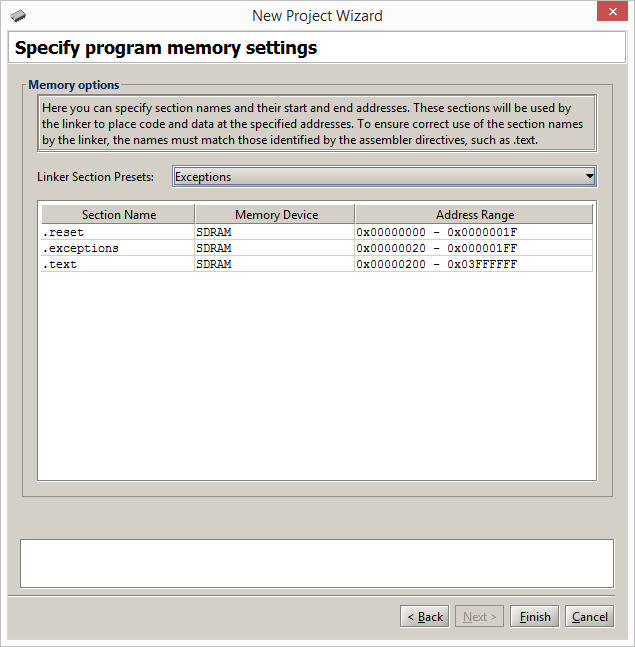
\includegraphics[scale=0.58]{figures/exceptions.png}
	\end{center}
	\vspace{-0.25cm}\caption{Selecting the {\sf Exceptions} linker section.}
\label{fig:exceptions}
\end{figure}

\newpage
\section*{ Part II}
\addcontentsline{toc}{2}{Part II}
Consider the main program shown in Figure~\ref{fig:code2}. The code is required to set up 
the Nios~II stack pointer and to enable interrupts from two sources: the pushbutton KEYs
and the Interval Timer.  The main program calls the subroutines {\it CONFIG\_TIMER} and 
{\it CONFIG\_KEYS} to set up the two ports. You are to write each of these subroutines. Set 
up the Interval Timer to generate one interrupt every 0.25 seconds.

~\\
In Figure~\ref{fig:code2} the main program executes an endless loop writing the value of
the global variable {\it COUNT} to the red lights LEDR.  In the interrupt service routine for 
the Interval Timer you are to increment the variable {\it COUNT} 
by the value of the {\it RUN} global variable, 
which should be either 1 or 0.  You are to toggle the value of the {\it RUN} global variable 
in the interrupt service routine for the pushbutton KEYs, each time a KEY is pressed.
When {\it RUN} = 0, the main program will display a static count on the red lights,
and when {\it RUN} = 1, the count shown on the red lights will increment every 0.25 seconds.

~\\
Make a new Monitor Program project for this part, and assemble, download, and test your
code.


\section*{ Part III}
\addcontentsline{toc}{3}{Part III}
Modify your program from Part II so that you can vary the speed at which the counter
displayed on the red lights is incremented. All of your changes for this part should be made
in the interrupt service routine for the pushbutton KEYs. The main program and the rest of
your code should not be changed.

~\\
Implement the following behavior. When {\it KEY}$_0$ is pressed, the value of the {\it RUN}
variable should be toggled, as in Part I. Hence, pressing {\it KEY}$_0$ stops/runs
the incrementing of the {\it COUNT} variable. When {\it KEY}$_1$ is pressed, the rate at which
{\it COUNT} is incremented should be either increased or decreased depending on the value of {\it SW}$_0$.
If {\it SW}$_0$ is 1, then the rate should be doubled, otherwise the
rate should be halved. You should implement this feature by stopping the Interval Timer within
the pushbutton KEYs interrupt service routine, modifying the load value used in the
timer, and then restarting the timer.

\section*{ Part IV}
\addcontentsline{toc}{4}{Part IV}
For this part you are to create a real-time clock that is shown on the seven-segment displays {\it HEX}$3-0$.
Set up an interval timer to provide an interrupt every 1/100 of a second. Use this
timer to increment a global variable called {\it TIME}. You should use the {\it TIME} variable as your real time clock.
Use the format \red{SS}:\red{DD}, where \red{\it SS} are seconds and \red{\it DD} are hundredths of a second.
When the clock reaches \red{59}:\red{99}, it should wrap around to \red{00}:\red{00}.

~\\
Make a new folder to hold your Monitor Program project for this part. Write the program for the
real-time clock. To show the {\it TIME} variable in the real-time clock format
\red{SS}:\red{DD}, you can use the same approach that was followed for Part 4 of Lab Exercise 4.
In that previous exercise you used polled I/O with the Interval Timer,
whereas now you are using interrupts. One possible way to structure your code is illustrated in
Figure~\ref{fig:code3}. The endless loop in this code writes the value of a variable named
{\it HEX\_code} to the {\it HEX}$3-0$ displays.

~\\
Using the scheme in Figure~\ref{fig:code3}, the interrupt service routine for the second 
Interval Timer has to increment the {\it TIME} variable, and also update
the {\it HEX\_code} variable that is being written to the 7-segment displays by the main program.

~\\
Make a new Monitor Program project and test your program. 
~\\

\begin{figure}[H]
\begin{center}
\lstinputlisting[style=defaultNiosStyle]{../design_files/part2.s}
\end{center}
\caption{Main program for Part II.}
\label{fig:code2}
\end{figure}

\begin{figure}[H]
\begin{center}
\lstinputlisting[style=defaultNiosStyle]{../design_files/part4.s}
\end{center}
\vspace{-0.5cm}\caption{Main program for Part IV.}
\label{fig:code3}
\end{figure}


%%%%%%%%%%%%%%%%%%%%%%%%%%%%%%%%%%%%%%%%
%%% FPGAcademy Copyright Information %%%
%%%%%%%%%%%%%%%%%%%%%%%%%%%%%%%%%%%%%%%%

%Always put the copyright on a new page (clear page), with some vertical space from top
\clearpage
\vspace{1in}

\noindent

Copyright {\copyright} FPGAcademy.org. All rights reserved. FPGAcademy and the 
FPGAcademy logo are trademarks of FPGAcademy.org.  This document is provided 
"as is", without warranty of any kind, express or implied, including but not 
limited to the warranties of merchantability, fitness for a particular purpose 
and noninfringement. In no event shall the authors or copyright holders be 
liable for any claim, damages or other liability, whether in an action of 
contract, tort or otherwise, arising from, out of or in connection with the 
document or the use or other dealings in the document.
~\\
~\\
**Other names and brands may be claimed as the property of others.


\end{document}
